\documentclass[landscape,a0,plainboxedsections]{sciposter}

\usepackage{amsmath}
\usepackage{amsfonts}
\usepackage{graphicx}
\usepackage{IEEEtrantools}
\usepackage{multicol}
\usepackage{algorithmic}
\usepackage{setspace}

\usepackage{tikz}
\usepackage{pgfplots}
 \usetikzlibrary{plotmarks}
 \pgfplotsset{compat=newest}
 \pgfplotsset{plot coordinates/math parser=false}
% \usepgfplotslibrary{external}
% \tikzexternalize[prefix=tikz/]

 
\title{Particle Gibbs with Refreshed Backward Simulation}
\author{Pete Bunch \qquad Fredrik Lindsten \qquad Sumeetpal Singh}
\institute{Department of Engineering, University of Cambridge, Trumpington Street, Cambridge, CB2 1PZ, UK}
\email{\{pb404,fsml2,sss40\}@cam.ac.uk}
\leftlogo[1.5]{CUnibig.pdf}


\newcommand{\meta}[1]{{\color{red}\em #1}}

\setmargins[3.5cm]
\setlength{\intextsep}{20\baselineskip plus 0.2\baselineskip minus 0.2\baselineskip}


%%%%%%%%%%%%%%%%%%%%%%%%%%%%%%%%%%%%%%%%%%%%%%%%%%%%%%%%%%%%%%%
%%% MACROS %%%
\newcommand{\ti}{t}
\newcommand{\timax}{T}

\newcommand{\pr}{\theta}
\newcommand{\prspace}{\Theta}

\newcommand{\ls}[1]{x_{#1}}
\newcommand{\lsspace}{\mathcal{X}}

\newcommand{\ob}[1]{y_{#1}}
\newcommand{\obspace}{\mathcal{Y}}

\newcommand{\nc}{Z}

\newcommand{\toas}{\stackrel{\text{a.s.}}{\to}}
\newcommand{\testfunc}{\zeta}
\newcommand{\prob}{P}

\newcommand{\id}[1]{q_{#1}}

\newcommand{\an}[1]{a_{#1}}
\newcommand{\ai}[1]{b_{#1}}
\newcommand{\notai}[1]{-b_{#1}}
\newcommand{\aifinal}{K}
\newcommand{\lsset}[1]{\mathbf{x}_{#1}}
\newcommand{\anset}[1]{\mathbf{a}_{#1}}

\newcommand{\den}{p}
\newcommand{\ed}{\pi}
\newcommand{\td}[1]{f_{\theta,#1}}
\newcommand{\od}[1]{g_{\theta,#1}}
\newcommand{\pd}[1]{\phi_{#1}}
\newcommand{\spd}[1]{\psi_{#1}}

\newcommand{\pw}[1]{w_{#1}}
\newcommand{\ppw}[1]{v_{#1}}
\newcommand{\spw}[1]{u_{#1}}

\newcommand{\mhap}{\alpha}
\newcommand{\pss}[1]{^{(#1)}}
\newcommand{\nump}{N}
\newcommand{\utf}[1]{\rho_{#1}}
\newcommand{\cised}{\eta}
\newcommand{\cisi}{c}
\newcommand{\notcisi}{-c}

\newcommand{\wl}{L}
%%%%%%%%%%%%%%%%%%%%%%%%%%%%%%%%%%%%%%%%%%%%%%%%%%%%%%%%%%%%%%%



\begin{document}
\maketitle
\begin{multicols}{4}

\section{Summary}
Particle Gibbs is a Markov Chain Monte Carlo algorithm which can be used for Bayesian parameter learning with Markovian state space models. It uses a particle filter at each iteration to sample a new state trajectory. The basic formulation often requires large numbers of particles in order to mix well, because of particle filter degeneracy. This problem can be mitigated by including a backward simulation sweep to increase the probability of changing the particle ancestry. Here we show how a modification to the backward simulation phase, in which new states are sampled simultaneously with the ancestor indexes, can further improve mixing.
%
%
%
\section{Preliminaries}
\paragraph*{Markovian state space model}
\begin{itemize}
 \item Sequence of latent states $\ls{\ti} \in \lsspace : \ti = 1,\dots,\timax$
 \item Sequence of observations $\ob{\ti} \in \obspace : \ti = 1,\dots,\timax$
 \item Model parameters $\pr \in \prspace$ with prior density $\den(\pr)$
 \item Model densities exist and depend on the parameters:
\end{itemize}
\begin{IEEEeqnarray}{rClcrCl}
 \ls{\ti}|\ls{\ti-1} & \sim & \td{\ti}(\ls{\ti}|\ls{\ti-1}) & \qquad & \ob{\ti}|\ls{\ti}   & \sim & \od{\ti}(\ob{\ti}|\ls{\ti})   \nonumber
\end{IEEEeqnarray}
\begin{itemize}
 \item The objective is to approximate the joint posterior density over all the unknown variables (with normalising constant $\nc$):
\end{itemize}
\begin{IEEEeqnarray}{rCl}
 \den(\pr, \ls{1:\timax} | \ob{1:\timax}) & = & \frac{1}{\nc} \cdot \den(\pr) \prod_{\ti=1}^{\timax} \od{\ti}(\ob{\ti}|\ls{\ti}) \td{\ti}(\ls{\ti}|\ls{\ti-1}) \label{eq:full-posterior}
\end{IEEEeqnarray}
\begin{itemize}
 \item An ideal Gibbs Sampler would target this by alternately sampling the conditionals $\den(\ls{1:\timax}|\pr,\ob{1:\timax})$ and $\den(\pr|\ls{1:\timax},\ob{1:\timax})$.
 \item Parameter conditional can be sampled directly or targeted with Metropolis-Hastings. State conditional is generally intractable.
\end{itemize}
%
%
%
\paragraph*{Particle Filter}
\begin{itemize}
 \item Recursively approximates the sequence of joint filtering densities $\den(\ls{1:\ti}|\pr,\ob{1:\ti})$ using $\nump$ particles, each one a weighted realisation of the state sequence:
\end{itemize}
\begin{IEEEeqnarray}{rCl}
 \{\ls{1:\ti}\pss{i}, \:\: \pw{\ti}\pss{i} \:\: : \:\: i = 1,\dots,\nump\} \nonumber
\end{IEEEeqnarray}
\begin{itemize}
 \item For each $\ti,i$, sample ancestor $\an{\ti}\pss{i} \in \{1,\dots,\nump\}$ and state $\ls{\ti}\pss{i}$ from:
\end{itemize}
\begin{IEEEeqnarray}{rCl}
 \frac{ \pw{\ti-1}\pss{\an{\ti}\pss{i}} }{ \sum_j \pw{\ti-1}\pss{j} } \: \id{\ti}(\ls{\ti}|\ls{\ti-1}\pss{\an{\ti}\pss{i}}) \nonumber
\end{IEEEeqnarray}
\begin{itemize}
 \item Update trajectory and weight:
\end{itemize}
\begin{IEEEeqnarray}{rClCrCl}
 \ls{1:\ti}\pss{i} & = & \ls{1:\ti-1}\pss{\an{\ti}\pss{i}} \: \cup \: \ls{\ti}\pss{i} & \qquad\qquad & \pw{\ti}\pss{i}   & = & \frac{ \td{\ti}(\ls{\ti}\pss{i}|\ls{\ti-1}\pss{\an{\ti}\pss{i}})\od{\ti}(\ob{\ti}|\ls{\ti}\pss{i}) }{ \id{\ti}(\ls{\ti}\pss{i}|\ls{\ti-1}\pss{\an{\ti}\pss{i}}) } \nonumber
\end{IEEEeqnarray}
\begin{itemize}
 \item Exhibits path-space degeneracy, a significant deficiency. Not all particles are propagated to the next time instant. The number of unique states appearing in the trajectories decreases as we look back in time.
\end{itemize}
%
%
%
\vfill
\columnbreak
\section{Particle Gibbs}
\begin{itemize}
 \item Consider all the random variable comprising a particle filter:
\end{itemize}
\begin{IEEEeqnarray}{rClCrClCl}
 \lsset{\ti} = \{\ls{\ti}\pss{i}\}_{i=1}^{\nump} & \quad,\quad & \anset{\ti} = \{\an{\ti}\pss{i}\}_{i=1}^{\nump} & \quad,\quad & \ti = 2,\dots,\timax \nonumber
\end{IEEEeqnarray}
\begin{itemize}
 \item Let $\aifinal\in\{1,\dots,\nump\}$ be the index of one particular reference trajectory, with ancestry:
\end{itemize}
\begin{IEEEeqnarray}{rCl}
 \ai{\ti} &=& \begin{cases}
               \aifinal & \ti = \timax \\
               \an{\ti+1}\pss{\ai{\ti+1}} & \ti = \timax-1,\dots,1
              \end{cases} \nonumber
\end{IEEEeqnarray}
\begin{itemize}
 \item Construct extended target distribution over all all these variables:
\end{itemize}
\begin{IEEEeqnarray}{rCl}
 \IEEEeqnarraymulticol{3}{l}{ \ed(\pr, \anset{2:\timax}, \lsset{1:\timax}, \aifinal) = \frac{1}{\nump^\timax} \cdot \den(\pr, \ls{1:\timax}\pss{\ai{1:\timax}}|\ob{1:\timax}) }\nonumber \\
  \qquad \times \prod_{i\ne\ai{1}} \id{1}(\ls{1}\pss{i}) \prod_{\ti=2}^{\timax} \left[ \prod_{i\ne\ai{\ti}} \frac{ \pw{\ti-1}\pss{\an{\ti}\pss{i}} }{ \sum_j \pw{\ti-1}\pss{j} } \id{\ti}(\ls{\ti}\pss{i}|\ls{\ti-1}\pss{\an{\ti}\pss{i}}) \right] \label{eq:extended_dist_v1}
\end{IEEEeqnarray}
\begin{itemize}
 \item This may be targeted without approximation, and admits the desired posterior as a marginal. \cite{Andrieu2010}
\end{itemize}
\begin{itemize}
 \item Sample alternately from conditional distributions for:
 \begin{itemize}
  \item $\pr$ (as before)
  \item $\{\anset{2:\timax}\pss{\notai{2:\timax}}, \lsset{1:\timax}\pss{\notai{1:\timax}}\}$ (conditional particle filter)
  \item $\aifinal$ (Sample from final set of weights)
 \end{itemize}
\end{itemize}
%
%
%
\section{Particle Gibbs with Backward Simulation}
\begin{itemize}
 \item Particle Gibbs mixing can be very slow, due to path-space degeneracy of conditional particle filter. Successive reference trajectories are likely to have a near-identical ancestry.
 \item Mitigated by backward simulation, an extra sampling stage to modify ancestors one at a time, instead of all at once. \cite{Godsill2004,Whiteley2010b}
 \item Sample new reference ancestor index for each $\ti$ (backwards in time) from:
\end{itemize}
\begin{IEEEeqnarray}{rCl}
 \ed(\an{\ti}\pss{\ai{\ti}} | \pr, \anset{2:\ti-1}, \lsset{1:\ti-1}, \an{\ti+1:\timax}\pss{\ai{\ti+1:\timax}}, \ls{\ti:\timax}\pss{\ai{\ti:\timax}}, \aifinal) & = & \frac{ \pw{\ti-1}\pss{\an{\ti}\pss{\ai{\ti}}} \td{\ti}(\ls{\ti}\pss{\ai{\ti}}|\ls{\ti-1}\pss{\an{\ti}\pss{\ai{\ti}}}) }{ \sum_j \pw{\ti-1}\pss{j} \td{\ti}(\ls{\ti}\pss{\ai{\ti}}|\ls{\ti-1}\pss{j}) } \nonumber \\ \label{eq:bs-distn}
\end{IEEEeqnarray}
\begin{itemize}
 \item This is a collapsed Gibbs move. \cite{Dyk2008} Future variables of reference trajectory are marginalised.
\end{itemize}
%
%
%
\section{Refreshed Backward Simulation}
\begin{itemize}
 \item Backward simulation is ineffective if the transition density is informative (low variance). See Figure~\ref{fig:bs-fail}.
 \item Improve mixing by simultaneously sampling new state(s) along with each ancestor index:
\end{itemize}
\begin{IEEEeqnarray}{l}
 \ed(\an{\ti}\pss{\ai{\ti}}, \ls{\ti}\pss{\ai{\ti}} | \pr, \anset{2:\ti-1}, \lsset{1:\ti-1}, \an{\ti+1:\timax}\pss{\ai{\ti+1:\timax}}, \ls{\ti+1:\timax}\pss{\ai{\ti+1:\timax}}, \aifinal) \nonumber \\
 \qquad\qquad = \frac{ \pw{\ti-1}\pss{\an{\ti}\pss{\ai{\ti}}} \td{\ti}(\ls{\ti}\pss{\ai{\ti}}|\ls{\ti-1}\pss{\an{\ti}\pss{\ai{\ti}}}) \od{\ti}(\ob{\ti}|\ls{\ti}\pss{\ai{\ti}}) \td{\ti+1}(\ls{\ti+1}\pss{\ai{\ti+1}}|\ls{\ti}\pss{\ai{\ti}}) }{ \sum_j \pw{\ti-1}\pss{j} \int \td{\ti}(\ls{}|\ls{\ti-1}\pss{j}) \od{\ti}(\ob{\ti}|\ls{}) \td{\ti+1}(\ls{\ti+1}\pss{\ai{\ti+1}}|\ls{}) d\ls{} } \label{eq:rbs-distn}
\end{IEEEeqnarray}
\begin{figure}
 \centering
 % This file was created by matlab2tikz v0.4.4 running on MATLAB 8.3.
% Copyright (c) 2008--2013, Nico Schlömer <nico.schloemer@gmail.com>
% All rights reserved.
% 
% The latest updates can be retrieved from
%   http://www.mathworks.com/matlabcentral/fileexchange/22022-matlab2tikz
% where you can also make suggestions and rate matlab2tikz.
% 
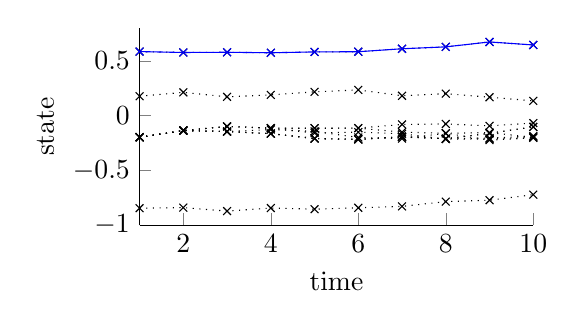
\begin{tikzpicture}

\begin{axis}[%
width=5cm,
height=2.5cm,
scale only axis,
xmin=1,
xmax=10,
xlabel={time},
ymin=-1,
ymax=0.8,
ylabel={state},
axis x line*=bottom,
axis y line*=left
]
\addplot [
color=black,
dotted,
mark=x,
mark options={solid},
forget plot
]
table[row sep=crcr]{
1 -0.845551240007797\\
2 -0.840546836824192\\
3 -0.872080048601409\\
4 -0.84421796719701\\
5 -0.854586924446221\\
6 -0.841810994872285\\
7 -0.829125183937655\\
8 -0.785553434570018\\
9 -0.772567675543346\\
10 -0.721980380882537\\
};
\addplot [
color=black,
dotted,
mark=x,
mark options={solid},
forget plot
]
table[row sep=crcr]{
1 0.178380225849766\\
2 0.213635363813657\\
3 0.172602954084374\\
4 0.190323850620537\\
5 0.218110342445606\\
6 0.235939570950501\\
7 0.182347219287174\\
8 0.201721962940765\\
9 0.169159051260375\\
10 0.136247215714753\\
};
\addplot [
color=black,
dotted,
mark=x,
mark options={solid},
forget plot
]
table[row sep=crcr]{
1 -0.196861446475943\\
2 -0.13598664093345\\
3 -0.144762690908006\\
4 -0.163836263043423\\
5 -0.208286519393592\\
6 -0.21658046659277\\
7 -0.192099174161813\\
8 -0.210809496440697\\
9 -0.160385450854037\\
10 -0.102479059666698\\
};
\addplot [
color=black,
dotted,
mark=x,
mark options={solid},
forget plot
]
table[row sep=crcr]{
1 -0.196861446475943\\
2 -0.13598664093345\\
3 -0.144762690908006\\
4 -0.163836263043423\\
5 -0.208286519393592\\
6 -0.21658046659277\\
7 -0.192099174161813\\
8 -0.210809496440697\\
9 -0.160385450854037\\
10 -0.102479059666698\\
};
\addplot [
color=black,
dotted,
mark=x,
mark options={solid},
forget plot
]
table[row sep=crcr]{
1 -0.196861446475943\\
2 -0.13598664093345\\
3 -0.144762690908006\\
4 -0.163836263043423\\
5 -0.208286519393592\\
6 -0.21658046659277\\
7 -0.192099174161813\\
8 -0.209956267108274\\
9 -0.204663908882357\\
10 -0.185975824479738\\
};
\addplot [
color=black,
dotted,
mark=x,
mark options={solid},
forget plot
]
table[row sep=crcr]{
1 -0.196861446475943\\
2 -0.13598664093345\\
3 -0.144762690908006\\
4 -0.126662292522634\\
5 -0.143404026783185\\
6 -0.199131513361006\\
7 -0.208977769655281\\
8 -0.160638059039865\\
9 -0.222781247847953\\
10 -0.203062717823216\\
};
\addplot [
color=black,
dotted,
mark=x,
mark options={solid},
forget plot
]
table[row sep=crcr]{
1 -0.196861446475943\\
2 -0.13598664093345\\
3 -0.0978611879077818\\
4 -0.113918626941059\\
5 -0.114772220288179\\
6 -0.113550295935696\\
7 -0.149987264343326\\
8 -0.160457205702751\\
9 -0.15412452565722\\
10 -0.198026028555778\\
};
\addplot [
color=black,
dotted,
mark=x,
mark options={solid},
forget plot
]
table[row sep=crcr]{
1 -0.196861446475943\\
2 -0.13598664093345\\
3 -0.0978611879077818\\
4 -0.113918626941059\\
5 -0.114772220288179\\
6 -0.113550295935696\\
7 -0.0801953097596561\\
8 -0.0752702852114935\\
9 -0.0927557198879093\\
10 -0.0671376566914904\\
};
\addplot [
color=black,
dotted,
mark=x,
mark options={solid},
forget plot
]
table[row sep=crcr]{
1 -0.196861446475943\\
2 -0.13598664093345\\
3 -0.0978611879077818\\
4 -0.113918626941059\\
5 -0.158207397501362\\
6 -0.149718292186502\\
7 -0.164943200831398\\
8 -0.214040513386765\\
9 -0.213495448093993\\
10 -0.196080777555403\\
};
\addplot [
color=black,
dotted,
mark=x,
mark options={solid},
forget plot
]
table[row sep=crcr]{
1 0.586442621667069\\
2 0.578187904446798\\
3 0.580168184685444\\
4 0.57551577312066\\
5 0.583282771835473\\
6 0.585189608414548\\
7 0.61215152299557\\
8 0.629592489655878\\
9 0.674435829442097\\
10 0.646877800107992\\
};
\addplot [
color=blue,
solid,
mark=x,
mark options={solid},
forget plot
]
table[row sep=crcr]{
1 0.586442621667069\\
2 0.578187904446798\\
3 0.580168184685444\\
4 0.57551577312066\\
5 0.583282771835473\\
6 0.585189608414548\\
7 0.61215152299557\\
8 0.629592489655878\\
9 0.674435829442097\\
10 0.646877800107992\\
};
\end{axis}
\end{tikzpicture}%
 \caption{A backward simulation sweep does not result in any changes to the reference particle ancestry (blue).}
 \label{fig:bs-fail}
\end{figure}
\begin{itemize}
 \item No change to extended target distribution.
 \item Intuitively, sample state so as to bridge the gap between discontinuous past and future.
 \item Easily extended to multiple time instants (i.e. sample $\ls{\ti:\ti+L-1}\pss{i}$).
\end{itemize}
%
%
%
\section{Markov Kernels for Refreshed Sampling}
\begin{itemize}
 \item Cannot sample \eqref{eq:rbs-distn} directly (continuous-discrete). Instead target with a Markov kernel.
 \item Write \eqref{eq:rbs-distn} in simplified form:
\end{itemize}
\begin{IEEEeqnarray}{rCl}
\ed(\an{\ti},\ls{\ti} | \lsset{\ti-1}) & = & \frac{ \pw{\ti-1}\pss{\an{\ti}} \utf{\ti}(\ls{\ti}|\ls{\ti-1}\pss{\an{\ti}}) }{ \sum_j \pw{\ti-1}\pss{j} \int \utf{\ti}(\ls{}|\ls{\ti-1}\pss{j}) d\ls{} } \label{eq:simplified-rbs-distn}
\end{IEEEeqnarray}
\begin{itemize}
 \item Can be targeted with Metropolis-Hastings (as in \cite{Bunch2012} for state smoothing).
 \item Alternatively, use conditional importance sampling. Particle Gibbs principle applied to a single time instant using extended target:
\end{itemize}
\begin{IEEEeqnarray}{rCl}
 \cised(\anset{\ti}, \lsset{\ti}, \cisi) & = & \frac{1}{\nump} \ed(\ls{\ti}\pss{\cisi}, \an{\ti}\pss{\cisi} | \lsset{\ti-1}) \prod_{i\ne\cisi} \frac{\ppw{\ti}\pss{\an{\ti}\pss{i}}}{\sum_j \ppw{\ti}\pss{j}} \spd{\ti}(\ls{\ti}\pss{i}|\ls{\ti-1}\pss{\an{\ti}\pss{i}}) \nonumber     . 
\end{IEEEeqnarray}
\parbox{0.9\columnwidth}{
\begin{algorithm}
\begin{algorithmic}[1]
\linespread{1.5} \selectfont
 \REQUIRE Preceding particle states $\lsset{\ti-1}$, current values $\{\an{\ti}^*,\ls{\ti}^*\}$.
 \STATE Sample an index uniformly $\cisi^*\in\{1,\dots,\nump\}$.
 \STATE Set $\an{\ti}\pss{\cisi^*} = \an{\ti}^*$. Set $\ls{\ti}\pss{\cisi^*} = \ls{\ti}^*$.
 \FORALL{$i \in \{1,\dots,\nump\}\setminus\cisi^*$}
  \STATE Sample $\an{\ti}\pss{i} \sim \frac{\ppw{\ti-1}\pss{\an{\ti}}}{\sum_j \ppw{\ti-1}\pss{j}}$. Sample $\ls{\ti}\pss{i} \sim \spd{\ti}(\ls{\ti}|\ls{\ti-1}\pss{\an{\ti}\pss{i}})$.
 \ENDFOR
 \STATE Sample $\cisi' \sim \frac{\spw{\ti}\pss{\cisi}}{\sum_j \spw{\ti}\pss{j}}$, where $\spw{\ti} = \frac{ \pw{\ti-1}\pss{\an{\ti}\pss{i}} \utf{\ti}(\ls{\ti}\pss{i}|\ls{\ti-1}\pss{\an{\ti}\pss{i}}) }{ \ppw{\ti-1}\pss{\an{\ti}\pss{i}} \spd{\ti}(\ls{\ti}\pss{i}|\ls{\ti-1}\pss{\an{\ti}\pss{i}}) }$.
 \STATE Set $\an{\ti}' = \an{\ti}\pss{\cisi'}$. Set $\ls{\ti}' = \ls{\ti}\pss{\cisi'}$.
 \RETURN New values $\{\an{\ti}',\ls{\ti}'\}$.
\end{algorithmic}
\caption[0.9]{Conditional importance sampling for the joint ancestor-state conditional distributions.}
\label{alg:cis}
\end{algorithm} }
%
%
%
\section{Simulations}
\begin{itemize}
 \item Tested on a tracking problem. Near constant velocity transition model (3D) with observations of bearing, elevation and range. Unknown scale factor on the transition covariance matrix.
 \item $5$ simulated data sets each of $100$ time steps. $5000$ MCMC iterations ($1000$ burn in).
 \item Compared particle Gibbs (PG), with ordinary (PG-BS) and refreshed (PG-RBS) backward simulation, varying number of particles.
 \item PG-RBS with $100$ particles takes same time as PG-BS with $200$.
 \item PG does not work (no convergence).
% \item EKF approximations to optimal importance densities wherever appropriate.
% \item PG-RBS used conditional importance sampling kernel with $\ppw{\ti}\pss{i}=\pw{\ti}\pss{i}$.
\end{itemize}

\begin{figure}
\centering
\subfigure[{\small PG-BS ($N=100$)}]{ % This file was created by matlab2tikz v0.4.4 running on MATLAB 8.3.
% Copyright (c) 2008--2013, Nico Schlömer <nico.schloemer@gmail.com>
% All rights reserved.
% 
% The latest updates can be retrieved from
%   http://www.mathworks.com/matlabcentral/fileexchange/22022-matlab2tikz
% where you can also make suggestions and rate matlab2tikz.
% 
%
% defining custom colors
\definecolor{mycolor1}{rgb}{0,0,0.5625}%
%
\begin{tikzpicture}

\begin{axis}[%
width=4.5cm,
height=4.5cm,
area legend,
scale only axis,
xmin=0.5,
xmax=2,
xlabel={$\sigma^2$},
ymin=0,
ymax=500,
axis x line*=bottom,
axis y line*=left
]
\addplot[ybar,bar width=0.170085103120214cm,draw=black,fill=mycolor1] plot coordinates{(0.710612054054637,26)
(0.761637584990702,67)
(0.812663115926766,118)
(0.86368864686283,196)
(0.914714177798895,271)
(0.965739708734959,390)
(1.01676523967102,394)
(1.06779077060709,410)
(1.11881630154315,390)
(1.16984183247922,351)
(1.22086736341528,308)
(1.27189289435134,274)
(1.32291842528741,195)
(1.37394395622347,145)
(1.42496948715954,101)
(1.4759950180956,81)
(1.52702054903167,56)
(1.57804607996773,47)
(1.62907161090379,31)
(1.68009714183986,34)
(1.73112267277592,26)
(1.78214820371199,22)
(1.83317373464805,20)
(1.88419926558412,11)
(1.93522479652018,7)
(1.98625032745624,8)
(2.03727585839231,7)
(2.08830138932837,8)
(2.13932692026444,4)
(2.1903524512005,2)};

\addplot [
color=black,
solid,
forget plot
]
table[row sep=crcr]{
0.5 0\\
2 0\\
};
\addplot [
color=black,
dotted,
forget plot
]
table[row sep=crcr]{
1 0\\
1 500\\
};
\end{axis}
\end{tikzpicture}% }
\subfigure[{\small PG-BS ($N=200$)}]{ % This file was created by matlab2tikz v0.4.4 running on MATLAB 8.3.
% Copyright (c) 2008--2013, Nico Schlömer <nico.schloemer@gmail.com>
% All rights reserved.
% 
% The latest updates can be retrieved from
%   http://www.mathworks.com/matlabcentral/fileexchange/22022-matlab2tikz
% where you can also make suggestions and rate matlab2tikz.
% 
%
% defining custom colors
\definecolor{mycolor1}{rgb}{0,0,0.5625}%
%
\begin{tikzpicture}

\begin{axis}[%
width=4.5cm,
height=4.5cm,
area legend,
scale only axis,
xmin=0.5,
xmax=2,
xlabel={$\sigma^2$},
ymin=0,
ymax=500,
axis x line*=bottom,
axis y line*=left
]
\addplot[ybar,bar width=0.178998656193082cm,draw=black,fill=mycolor1] plot coordinates{(0.694917780309864,21)
(0.748617377167789,37)
(0.802316974025714,94)
(0.856016570883639,222)
(0.909716167741564,320)
(0.96341576459949,423)
(1.01711536145741,350)
(1.07081495831534,373)
(1.12451455517326,380)
(1.17821415203119,311)
(1.23191374888912,318)
(1.28561334574704,288)
(1.33931294260497,235)
(1.39301253946289,186)
(1.44671213632082,129)
(1.50041173317874,88)
(1.55411133003667,65)
(1.60781092689459,33)
(1.66151052375252,23)
(1.71521012061044,19)
(1.76890971746837,13)
(1.82260931432629,16)
(1.87630891118422,12)
(1.93000850804214,17)
(1.98370810490007,14)
(2.03740770175799,5)
(2.09110729861592,4)
(2.14480689547384,3)
(2.19850649233177,0)
(2.25220608918969,1)};

\addplot [
color=black,
solid,
forget plot
]
table[row sep=crcr]{
0.5 0\\
2 0\\
};
\addplot [
color=black,
dotted,
forget plot
]
table[row sep=crcr]{
1 0\\
1 500\\
};
\end{axis}
\end{tikzpicture}% }
\subfigure[{\small PG-RBS ($N=100$)}]{ % This file was created by matlab2tikz v0.4.4 running on MATLAB 8.3.
% Copyright (c) 2008--2013, Nico Schlömer <nico.schloemer@gmail.com>
% All rights reserved.
% 
% The latest updates can be retrieved from
%   http://www.mathworks.com/matlabcentral/fileexchange/22022-matlab2tikz
% where you can also make suggestions and rate matlab2tikz.
% 
%
% defining custom colors
\definecolor{mycolor1}{rgb}{0,0,0.5625}%
%
\begin{tikzpicture}

\begin{axis}[%
width=4.5cm,
height=4.5cm,
area legend,
scale only axis,
xmin=0.5,
xmax=2,
xlabel={$\sigma^2$},
ymin=0,
ymax=500,
axis x line*=bottom,
axis y line*=left
]
\addplot[ybar,bar width=0.135812392440373cm,draw=black,fill=mycolor1] plot coordinates{(0.607294061023861,4)
(0.648037778755973,4)
(0.688781496488085,29)
(0.729525214220197,36)
(0.77026893195231,105)
(0.811012649684422,155)
(0.851756367416534,249)
(0.892500085148646,291)
(0.933243802880758,337)
(0.973987520612871,369)
(1.01473123834498,329)
(1.0554749560771,355)
(1.09621867380921,314)
(1.13696239154132,290)
(1.17770610927343,254)
(1.21844982700554,185)
(1.25919354473766,172)
(1.29993726246977,128)
(1.34068098020188,120)
(1.38142469793399,100)
(1.4221684156661,51)
(1.46291213339822,42)
(1.50365585113033,25)
(1.54439956886244,20)
(1.58514328659455,13)
(1.62588700432667,9)
(1.66663072205878,7)
(1.70737443979089,3)
(1.748118157523,3)
(1.78886187525511,1)};

\addplot [
color=black,
solid,
forget plot
]
table[row sep=crcr]{
0.5 0\\
2 0\\
};
\addplot [
color=black,
dotted,
forget plot
]
table[row sep=crcr]{
1 0\\
1 500\\
};
\end{axis}
\end{tikzpicture}% }
\caption{Posterior histograms}
\label{fig:sample_hist}
\end{figure}
%
\begin{figure}
\centering
% This file was created by matlab2tikz v0.4.4 running on MATLAB 8.3.
% Copyright (c) 2008--2013, Nico Schlömer <nico.schloemer@gmail.com>
% All rights reserved.
% 
% The latest updates can be retrieved from
%   http://www.mathworks.com/matlabcentral/fileexchange/22022-matlab2tikz
% where you can also make suggestions and rate matlab2tikz.
% 
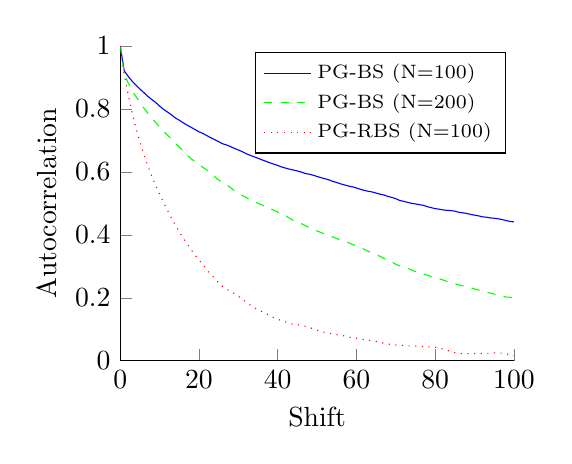
\begin{tikzpicture}

\begin{axis}[%
width=5cm,
height=4cm,
scale only axis,
xmin=0,
xmax=100,
xlabel={Shift},
ymin=0,
ymax=1,
ylabel={Autocorrelation},
axis x line*=bottom,
axis y line*=left,
legend style={draw=black,fill=white,legend cell align=left,font=\scriptsize}
]
\addplot [
color=blue,
solid
]
table[row sep=crcr]{
0 0.999903588398655\\
1 0.920486758741033\\
2 0.903335600089798\\
3 0.887932912664518\\
4 0.875071561743713\\
5 0.862746477492585\\
6 0.851314107455174\\
7 0.839539717987804\\
8 0.829617302754404\\
9 0.819980096411471\\
10 0.80851358299916\\
11 0.798425692380472\\
12 0.789661712034424\\
13 0.781040752052782\\
14 0.770955684745448\\
15 0.763721647120573\\
16 0.755612497589696\\
17 0.747979350271797\\
18 0.74125998446863\\
19 0.734015903212486\\
20 0.726885609263636\\
21 0.721774805650458\\
22 0.714834974081635\\
23 0.70817942947304\\
24 0.701898147848601\\
25 0.695616649427075\\
26 0.688974608321642\\
27 0.6851970987231\\
28 0.680062512922832\\
29 0.6742958539347\\
30 0.669354507938002\\
31 0.663801465676009\\
32 0.657324012584225\\
33 0.652239054507617\\
34 0.647495753789502\\
35 0.642939438890071\\
36 0.63803813715115\\
37 0.633199398445475\\
38 0.628545342669218\\
39 0.624336512986373\\
40 0.620238414860391\\
41 0.615311934916251\\
42 0.611695957499656\\
43 0.608310727704075\\
44 0.60550665634806\\
45 0.602463687990571\\
46 0.599238899231897\\
47 0.594598732631037\\
48 0.592495930677031\\
49 0.589200399894096\\
50 0.585110833142028\\
51 0.581402529342026\\
52 0.577920187311273\\
53 0.574500259063287\\
54 0.569415472560249\\
55 0.565955441292513\\
56 0.561673158412858\\
57 0.558083952812055\\
58 0.554806799771933\\
59 0.55219885880144\\
60 0.54844815006866\\
61 0.544501785509853\\
62 0.540985283756493\\
63 0.538066109300578\\
64 0.536001441562287\\
65 0.532198410435559\\
66 0.528996414229476\\
67 0.526309604928353\\
68 0.521589368070406\\
69 0.518658366353822\\
70 0.514465745513353\\
71 0.508946063401548\\
72 0.506226975519337\\
73 0.503134011096087\\
74 0.499868691306728\\
75 0.498066451993802\\
76 0.495571368463879\\
77 0.49355915035869\\
78 0.489197877917402\\
79 0.486131482756531\\
80 0.482969539462418\\
81 0.481372073527897\\
82 0.479024702393476\\
83 0.477740704816924\\
84 0.476640239654847\\
85 0.475103985782292\\
86 0.471327335736112\\
87 0.46968554058109\\
88 0.467853043993988\\
89 0.464760815570657\\
90 0.462341589505022\\
91 0.460176468560824\\
92 0.457070342540286\\
93 0.455870346197615\\
94 0.453600076942254\\
95 0.452398031197086\\
96 0.450827856118165\\
97 0.448215475094587\\
98 0.445449836835981\\
99 0.442224738235369\\
100 0.441071594680408\\
};
\addlegendentry{PG-BS (N=100)};

\addplot [
color=green,
dashed
]
table[row sep=crcr]{
0 0.999891622509946\\
1 0.9131246158294\\
2 0.882590227019065\\
3 0.8582602335872\\
4 0.83864457797386\\
5 0.820362545887663\\
6 0.802387098269211\\
7 0.786505235036271\\
8 0.770814721666268\\
9 0.757092639968614\\
10 0.742342348503673\\
11 0.728497879036039\\
12 0.716143443561847\\
13 0.703853923211808\\
14 0.691396752686264\\
15 0.677772859360532\\
16 0.666288650358538\\
17 0.653209238540924\\
18 0.641498206692758\\
19 0.632365913374451\\
20 0.622792424946645\\
21 0.614121802860441\\
22 0.60537280475484\\
23 0.594313485223001\\
24 0.583971860831792\\
25 0.573835170993497\\
26 0.566436191669736\\
27 0.558552263209654\\
28 0.549839340354118\\
29 0.540130464552977\\
30 0.532755589171176\\
31 0.524876622654475\\
32 0.51855139173525\\
33 0.511278961624043\\
34 0.506446429199656\\
35 0.499705126430569\\
36 0.494845992349021\\
37 0.488700271131707\\
38 0.484018516707596\\
39 0.478072697855192\\
40 0.472090833324776\\
41 0.466513223118886\\
42 0.460223428261561\\
43 0.452526218331281\\
44 0.445328368759231\\
45 0.440265398222439\\
46 0.435392297235818\\
47 0.428947618670154\\
48 0.423183579560225\\
49 0.417462989012893\\
50 0.411995013201967\\
51 0.407205932684084\\
52 0.402207830935458\\
53 0.397922306870715\\
54 0.393058219680795\\
55 0.387814257947974\\
56 0.383033023373619\\
57 0.378414999882359\\
58 0.374851280357911\\
59 0.369324121495941\\
60 0.364867272184509\\
61 0.359489327007041\\
62 0.353595077317804\\
63 0.347355069614687\\
64 0.341719696683109\\
65 0.336888527985878\\
66 0.331428006813312\\
67 0.324761659342965\\
68 0.319013074482997\\
69 0.313271440290862\\
70 0.306303817457784\\
71 0.301138009026498\\
72 0.297389379001777\\
73 0.29347833550842\\
74 0.288296196445506\\
75 0.282584345673744\\
76 0.279371813047442\\
77 0.275157239074421\\
78 0.272128280457854\\
79 0.267272972722048\\
80 0.264261166815676\\
81 0.260413975258518\\
82 0.256436206347447\\
83 0.251588116325574\\
84 0.248496252124085\\
85 0.243938512892472\\
86 0.241065536660925\\
87 0.238299602509428\\
88 0.235290538187007\\
89 0.232054998039984\\
90 0.227924449045455\\
91 0.224588471187677\\
92 0.221257774791747\\
93 0.217308396373018\\
94 0.215075613077136\\
95 0.211706605033252\\
96 0.207989158206567\\
97 0.206486957352932\\
98 0.202275599725738\\
99 0.201825138277393\\
100 0.199200058201334\\
};
\addlegendentry{PG-BS (N=200)};

\addplot [
color=red,
dotted
]
table[row sep=crcr]{
0 0.999836856429826\\
1 0.910398688836733\\
2 0.844782150614985\\
3 0.787620042324497\\
4 0.737853651209422\\
5 0.693994838677503\\
6 0.654315850392674\\
7 0.618568217625445\\
8 0.586195338684792\\
9 0.556818731672658\\
10 0.528109497284171\\
11 0.502829814719507\\
12 0.477350566982722\\
13 0.453688901611592\\
14 0.430564363314501\\
15 0.40897930305615\\
16 0.389484210518673\\
17 0.370964783991475\\
18 0.353018700995438\\
19 0.33540299548346\\
20 0.319933653980552\\
21 0.305356253628572\\
22 0.289179203425347\\
23 0.274406042861078\\
24 0.261304135708604\\
25 0.247755998137365\\
26 0.236061687396796\\
27 0.227463781647957\\
28 0.220244136793719\\
29 0.213287617224539\\
30 0.20490129570517\\
31 0.195880371291582\\
32 0.186137927637386\\
33 0.177132772427266\\
34 0.169414673416553\\
35 0.161318486645558\\
36 0.155992486114113\\
37 0.14976022437866\\
38 0.144525499746458\\
39 0.136632852447348\\
40 0.131445190441772\\
41 0.127907247448965\\
42 0.123132985717143\\
43 0.11952692899989\\
44 0.115364350672671\\
45 0.114805238457567\\
46 0.112324292775659\\
47 0.109479786360627\\
48 0.105858668864598\\
49 0.101598658448661\\
50 0.0969952588664834\\
51 0.0932471617431775\\
52 0.0900665289146602\\
53 0.0871118085891429\\
54 0.0850219392513513\\
55 0.0828455892510456\\
56 0.0814442204557225\\
57 0.0785079304935199\\
58 0.0747592673039743\\
59 0.0735481626352929\\
60 0.0716276326337509\\
61 0.069873210243891\\
62 0.0667399310572844\\
63 0.0649374977859129\\
64 0.0629298967091192\\
65 0.0611635809746716\\
66 0.058076033541349\\
67 0.0556469569111609\\
68 0.0533158867783404\\
69 0.0517332091355979\\
70 0.050111071873803\\
71 0.0498392679342351\\
72 0.048673904316628\\
73 0.0476411846370012\\
74 0.0471502717819124\\
75 0.046694203985966\\
76 0.0459429594082649\\
77 0.0450003431629298\\
78 0.0443270395112047\\
79 0.0443381644899684\\
80 0.0432467756119263\\
81 0.0414659584998818\\
82 0.0372622166510958\\
83 0.0334647377790083\\
84 0.0295848968740434\\
85 0.0259132126267024\\
86 0.0232463565628023\\
87 0.0222163617765922\\
88 0.0223982565101699\\
89 0.0228233732461777\\
90 0.0225172441669789\\
91 0.0228275365879988\\
92 0.0231265577263647\\
93 0.0230560657873127\\
94 0.0236575228549241\\
95 0.0252025267224022\\
96 0.023964658362867\\
97 0.024175673155557\\
98 0.0224850074230927\\
99 0.0186754976327629\\
100 0.0161258088535605\\
};
\addlegendentry{PG-RBS (N=100)};

\end{axis}
\end{tikzpicture}%
\caption{Mean autocorrelation function for PG-BS and PG-RBS.}
\label{fig:acf}
\end{figure}
\vspace{-2cm}
%
%
%
\section{Conclusions}
\begin{itemize}
 \item Simple but effective modification to standard PG-BS algorithm.
 \item States sampled simultaneously with ancestor indexes in backwards sweep.
 \item Direct sampling of conditional posterior not possible, but efficient Markov kernels exist.
 \item Improves mixing of Markov chain by increasing the probability of changing the ancestry.
 \item Can also be used with ancestor sampling \cite{Lindsten2014} instead of backward simulation.
\end{itemize}




{ \small
\bibliographystyle{IEEEbib}
\bibliography{/users/pete/Dropbox/PhD/Cleanbib}
% \bibliography{/home/pete/Dropbox/PhD/Cleanbib}
}
\vfill

\end{multicols}
\end{document}
